\chapter{Вёрстка таблиц}\label{ch:ch3}
\section{Квазилинейная систама уравнений для совместной эволюции вейбелевсой и ленгмюрвоской турбулентностей}

Для различных задач физики лабораторной и космической бесстолкновительной плазмы, включая солнечный ветер и магнитосферы звезд и планет, характерно наличие пучка энергичных заряженных частиц (электронов и/или ионов) в теплой плазме~\cite{Gary1993,Treumann1997,Marsch2006}. Даже если распределение частиц по скоростям в плазме и в пучке является изотропным максвелловским (в соответствующей  системе отсчета), для совместной системы "плазма+пучок" распределение будет анизотропным.  В результате, согласно дисперсионному анализу~\cite{Mikhailovsky1971,Fried1959,Krall1973,Tzoufras2006,Bret2010}, могут одновременно развиваться различные кинетические неустойчивости, прежде всего резонансная квазиэлектростатическая двухпотоковая неустойчивость и апериодическая квазимагнитостатическая неустойчивость вейбелевского типа, известные также как пучковая и филаментационная соответственно. 

Двухпотоковой неустойчивости подвержены продольные ленгмюровские (плазменные) волны, так что её развитие приводит к формированию коротковолновой ленгмюровской турбулентности электрического поля и плотности плазмы~\cite{Vedenov1963,Zakharov1972,VedenovRyutov1975,Krall1973,Appert1976,Yi2010,Bakunin2017,Sun2022}; при этом в общем распределении частиц образуется плато в области  скоростей между теплой плазмой и пучком.  Вследствие филаментационной неустойчивости возникает вейбелевская (магнитная) турбулентность, а именно, формируются более длинноволновые поперечные квазимагнитостатические поля и согласованные с ними токовые филаменты или слои~\cite{Weibel1959, Zhou2022,Fried1959, Kalman1968, Morse1971, Kocharovsky2016, Lazar2006, Stockem2009, SchaeferRolffs2006}; при этом уменьшается анизотропия общего распределения частиц по скоростям и его пучковая часть сглаживается.


Нас будет интересовать незамагниченная плазма, для которой двухпотоковая (пучкового типа) и филаментационная (вейбелевского типа) неустойчивости по отдельности изучены достаточно подробно, особенно в линейном приближении; см., например,~\cite{Mikhailovsky1971,Fried1959,Tzoufras2006,Hao2008,Bret2010,Moya2022}. При этом для исследования долговременной нелинейной динамики турбулентности, возникающей в результате развития изолированных двухпотоковой или филаментационной неустойчивостей, применялись как  полноценные расчеты методом частиц в ячейках~\cite{Kasaba2001,Dum1994,Yi2010,Ruyer2015,Dieckmann2009,Bret2010,Lazar2023,Nechaev2023,Kocharovsky2024,Garasev2022,Kuznetsov2025a}, так и различные приближенные подходы, прежде всего квазилинейные~\cite{Vedenov1963,VedenovRyutov1975,Appert1976,Bakunin2017,Ziebell2008,Lemons1979,Davidson1972,Ruyer2015,Kuznetsov2022,Kuznetsov2023}. 

Однако до сих пор слабо освещена проблема нелинейного взаимодействия ленгмюровской и вейбелевской турбулентности, важная для анализа таких явлений, как формирование бесстолкновительных ударных волн и структур в аккреционных дисках и колонках, взаимопроникновения соседних облаков и потоков частиц звёздного ветра, развитие корональных выбросов массы и солнечных вспышек, нагрев плазмы и изменение её кинетических свойств при инжекции пучков высокоэнергичных частиц и др.~\cite{Marcowith2016,Treumann2015,Aschwanden2005,Medvedev2006,Nishikawa2009,Kato2007,Kuznetsov2025b}. Имеющиеся выборочные работы в этом направлении исследований основаны преимущественно на расчетах методом частиц в ячейках, зачастую ограничиваются гидродинамическим режимом той или иной неустойчивости и по существу не касаются, а тем более не детализируют взаимное влияние ленгмюровской и вейбелевской  турбулентности; ср., например,~\cite{Kong2009,Ruyer2015,Bret2010,Lazar2023} (при наличии внешнего магнитного поля см. также работы~\cite{Lazar2023,Lopez2020}). Так, в обзоре~\cite{Bret2010}, являющемся, по-видимому, наиболее полным для интересующей нас задачи в отсутствие внешнего магнитного поля, обсуждаются условия насыщения и возможные нелинейные локализованные структуры в турбулентности каждого типа, но не изучается влияние изменения функции распределения частиц под действием турбулентности одного типа на развитие другой, хотя и упоминается возможность их последовательного развития.

В настоящей работе предпринято детальное изучение одного из механизмов взаимного влияния указанных неустойчивостей для кинетического режима их нарастания, насыщения и последующей релаксации сформировавшейся слабой турбулентности. А именно, проанализировано, как каждое из турбулентных полей - в основном электрическое или магнитное для двухпотоковой или филаментационной неустойчивостей соответственно - изменяет общую среднюю по пространству функцию распределения частиц по скоростям и тем самым модифицирует ход сопутствующей неустойчивости. В подобном квазилинейном подходе~\cite{VedenovRyutov1975,Appert1976,Kuznetsov2022,Kuznetsov2023} каждая мода турбулентности эволюционирует локально во времени согласно её инкременту (декременту), вычисляемому в линейном приближении с использованием указанной мгновенной функции распределения частиц. При этом рассматриваются условия, в которых, как подтверждают тестовые расчеты методом частиц в ячейках, исключена определяющая роль других возможных механизмов нелинейного изменения спектра обеих типов турбулентности, например, появление множественных ленгмюровских солитонов с нескомпенсированным зарядом или z-пинчей тока и систематическое трех- или четырехволновое взаимодействие отдельных мод (пространственных гармоник).

С этой целью построена замкнутая квазилинейная система уравнений, разработан оригинальный численный код её решения и с его помощью рассчитана одновременная нелинейная динамика большого числа (многих тысяч) ленгмюровских и вейбелевских мод турбулентной плазмы в кинетическом приближении, когда допустимые инкременты $\gamma$ и соответствующие волновые числа $k$ всех мод удовлетворяют неравенству $\gamma\ll kv_T$, где $v_T$~--- тепловая скорость. В результате установлена роль квазилинейного взаимодействия мод в эволюции спектров ленгмюровской и вейбелевской турбулентности, а также найдена динамика среднеквадратичных электрического и магнитного полей в ней и указан неравномерный характер уменьшения анизотропии распределения частиц по скоростям и увеличения тепловой энергии плазмы (нагрев) в поперечном к пучку направлении. 

Такой подход соответствует классическому квазилинейному описанию ленгмюровской турбулентности~\cite{VedenovRyutov1975,Appert1976} и развитому в работах~\cite{Kuznetsov2022,Kuznetsov2023} описанию турбулентности вейбелевского типа. Преимуществами подобного подхода перед моделированием методом частиц в ячейках являются возможность свободно выбирать диапазон представляющих интерес волновых векторов мод и регулировать начальный уровень их амплитуд. Это позволяет не только по отдельности верифицировать квазилинейное описание филаментационных и двухпотоковых мод путем сравнения получающихся частных результатов с найденными ранее результатами расчетов методом частиц в ячейках, но и сравнить независимую динамику спектра тех и других мод с их совместной динамикой. Немаловажной является и меньшая требовательность квазилинейных расчетов к вычислительным ресурсам, загруженность которых в расчетах методом частиц в ячейках оказывается многократно выше, в частности, из-за необходимости использования большого числа частиц  для корректного описания резонансных эффектов кинетической двухпотоковой неустойчивости~\cite{Lotov2015}.  

Для простоты представленные результаты ограничены решением начальной двумерной задачи для однородной незамагниченной нерелятивистской системы "плазма+пучок", в которой фоновая плазма и пучок включают холодные ионы и имеют одинаковую тепловую скорость $v_T$ (и температуру $T$) электронов, а направленная вдоль оси $y$ скорость пучка $v_s$ не сильно превышает тепловую скорость. В рассматриваемых условиях эффекты появления локализованного пространственного заряда и z-пинчевания токов плазмы отсутствуют~\cite{Tzoufras2006,Hao2008,Kocharovsky2024,Garasev2022}. Исследуется квазилинейная эволюция спектра  двухпотоковых (ленгмюровских) мод, т.е. фактически электростатических возмущений с волновыми векторами, в основном сонаправленными с пучком, и спектра филаментационных (вейбелевских) мод, т.е. поперечных электромагнитных возмущений с почти ортогональными пучку волновыми векторами~\cite{Bret2004,Bret2010}. Эти два спектра мод хорошо разделены по направлению и величинам волновых векторов и для их описания используются две прямоугольные сетки волновых векторов, плотно покрывающие область неустойчивости~(рис. \ref{fig:1}).  
\begin{figure}[h]

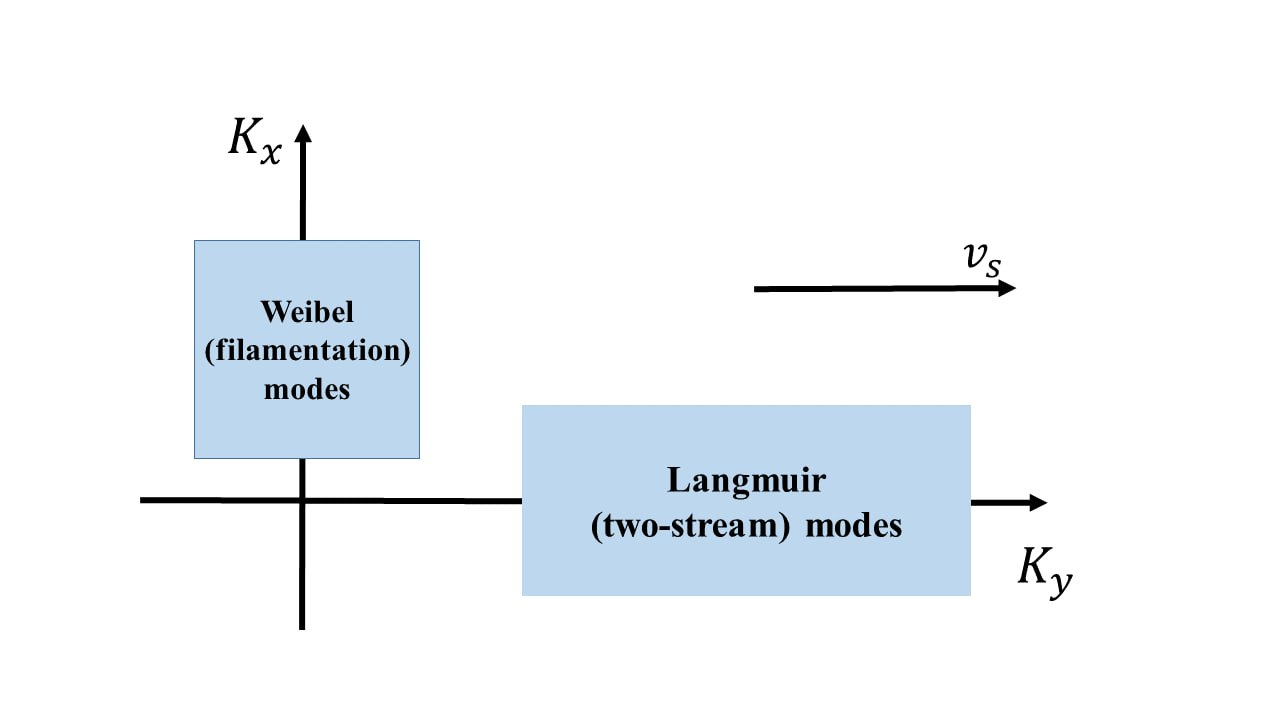
\includegraphics[width=1\linewidth]{part3/1.jpg}
\captionstyle{normal}
\caption{Схема расчетной плоскости, включающая две прямоугольные сетки волновых векторов для генерируемых спектров филаментационных и двухпотоковых мод.}
\label{fig:1}
\end{figure}

Квазилинейная система уравнений, используемая для моделирования, представлена в разделе 2. В разделах 3 и 4 обсуждаются результаты численных расчетов для двух характерных наборов параметров плазмы и пучка, отвечающих качественно различной динамике спектров мод. В заключении подводятся итоги и обсуждаются возможные направления дальнейших исследований.



Для бесстолкновительной плазмы, в которой на рассматриваемых временах порядка десяти времен насыщения неустойчивости можно пренебречь движением тяжелых ионов, самосогласованные уравнения Власова~-- Максвелла для функции распределения электронов $f(v_x , v_y , x, y, t)$, включающей их концентрацию $N (x, y, t)$, и электрического $\vec{E}=(E_x, E_y, 0)$ и магнитного $\vec{B}=(0, 0, B_z)$ полей имеют вид~\cite{Mikhailovsky1971,Krall1973,Baumjohann2012,Vedenov1963,VedenovRyutov1975,Bakunin2017,Kocharovsky2016}:
\begin{eqnarray}
    \dfrac{\partial f}{\partial t}+\vec{v}\dfrac{\partial f}{\partial \vec{r}}+\dfrac{e}{\me} \left(\vec{E}+\dfrac{1}{c}\left[\vec{v},\vec{B}\right]\right) \dfrac{\partial f}{\partial \vec{v}}=0, \\
    %
    \label{eq:maxw1} 
    \nabla \times \vec{B}=\dfrac{1}{c}\dfrac{\partial \vec{E}}{\partial t}+\dfrac{4\pi}{c}\vec{j}, \\
    %
    \label{eq:maxw2}
    \nabla \times \vec{E}=-\dfrac{1}{c}\dfrac{\partial \vec{B}}{\partial t},
\end{eqnarray}
где $c$~--- скорость света в вакууме, $e$ и $\me$~--- заряд и масса электрона, $\vec{j}=e\iint^{+\infty}_{-\infty}\vec{v}f(v_x , v_y , x, y, t) dv_x dv_y$~--- плотность тока, $N=\iint^{+\infty}_{-\infty}f(v_x , v_y , x, y, t)dv_xdv_y$ и учтено, что векторы координаты и скорости имеют только две компоненты, $\vec{r}=(x , y ,0)$ и $\vec{v}=(v_x , v_y ,0)$, согласно двумерной постановке задачи. 

При прохождении через фоновую плазму достаточно широкого пучка частиц, поперечный размер которого много больше плазменного скин-слоя, возникает обратный ток, так что $n_b\beta_{b}=n_s\beta_{s}$~\cite{Shukla2018,Jia2013,Karlick2008}, где $n_i$ и $\beta_i=v_i/c$~--- начальная концентрация и безразмерная направленная скорость фракций частиц: индексы $b$ и $s$ соответствуют фону и пучку. Поэтому используемое в работе обезразмеренное начальное распределение электронов по скоростям имеет вид
\begin{equation}
\label{eq:bp}
    \Psi_0(\vec{\beta})=\dfrac{n_b}{\pi\beta_T^2} \exp\left(-\dfrac{\beta_x^2}{\beta_T^2}-\dfrac{\left(\beta_y+\beta_{b}\right)^2}{\beta_T^2}\right)+\dfrac{n_s}{\pi\beta_T^2 } \exp\left(-\dfrac{\beta_x^2}{\beta_T^2}-\dfrac{\left(\beta_y-\beta_{s}\right)^2}{\beta_T^2}\right).  
\end{equation}
Выше $\beta_{x,y}={v_{x,y}}/{c}$, т.\,е. $\vec{\beta}=\vec{v}/{c}$, $\beta_T=\sqrt{2nk_bT/m_e}/c$, где включена постоянная Больцмана $k_b$. 

Квазилинейный подход к описанию взаимного влияния ленгмюровской и вейбелевской турбулентностей основан на разложении по пространственным модам решения уравнений  Максвелла~-- Власова~\cite{Baumjohann2012} с шумоподобным примерно равномерным по спектру начальным возмущением электромагнитного поля для мод филаментационной и двухпотоковой неустойчивостей. Такое разложение особенно эффективно тогда, когда ключевую роль играет интегральное нелинейное взаимодействие мод посредством их совместного изменения средней по пространству функции распределения частиц по скоростям. Последняя определяет текущие значения инкрементов (декрементов) и действительных частот всех рассматриваемых мод, в остальном эволюционирующих независимо. 
Подобное квазилинейное описание турбулентности оправдано в условиях случайности фаз мод и отсутствия захвата частиц электрическими или магнитными полями отдельных гармоник либо локализованных в пространстве структур, что обычно справедливо в кинетическом режиме развития неустойчивости и дальнейшей нелинейной динамики слабой турбулентности~\cite{GaleevSagdeev1969,Bakunin2017,Kuznetsov2023}. Наличие большого числа однотипных не сфазированных мод, достаточно плотно заполняющих значимую область волновых векторов, гарантирует гладкость формы и плавность изменения функции распределения частиц по скоростям, исключая артефакты когерентной интерференции и отрицательные значения этой функции всюду, кроме, возможно, несущественной, содержащей крайне мало частиц, области их скоростей, очень больших по сравнению с тепловыми скоростями. При этом по существу реализуется адиабатическая динамика каждой моды, непрерывно подстраивающейся к изменяющейся функции распределения электронов. 

В рассматриваемом двумерно-неоднородном случае для описания вейбелевской турбулентности используется сетка из часто расположенных и перекрывающих всю турбулентную область волновых векторов $m_W \cdot s_W$ неколлинеарных мод с хаотическими фазами и примерно одинаковыми исходными амплитудами при $t=0$. Аналогичная сетка $m_L \cdot s_L$ неколлиннеарных мод выбрана и для описания ленгмюровской турбулентности~(рис. \ref{fig:1}), где $m_i$ и $s_i$~--- количество заданных дискретных значений соответствующих ортогональных проекций $\vec{K}\vec{x_0}$ и $\vec{K}\vec{y_0}$ волновых векторов. В этом представлении магнитное поле имеет вид суммы по целочисленному векторному индексу $\vec{n}=(n_x,n_y)$:
\begin{equation}
    B_z(t,x,y)= \mathrm{Re} \Biggr[ \sum^{m_W,s_W}_{n_x,n_y=1}B_{k_\vec{n}}(t)\exp(- ik_{n_{x}}x - ik_{n_{y}}y)\Biggr]+ \mathrm{Re} \Biggr[\sum^{m_L,s_L}_{n_x,n_y=1}B_{k_\vec{n}}(t)\exp(- ik_{n_{x}}x - ik_{n_{y}}y)\Biggr].
\end{equation}
Аналогичный вид имеют обе компоненты электрического поля $E_x$ и $Ey$, а также возмущение 
функции распределения $\delta f(t,x,y)$. Получаемая из уравнений Власова-Максвелла квазилинейная система  $4(m_W\cdot s_W+m_L\cdot s_L)+1$ уравнений для усредненной в пространстве компоненты функции распределения электронов по скоростям $\psi_0$,  а также безразмерных комплексных амплитуд её возмущений $\psi_{K_{\vec{n}}}$ и возмущений магнитного $b_{K_{\vec{n}}}$ и двух компонент электрического  $e_{x{K_{\vec{n}}}}$ и $e_{y{K_{\vec{n}}}}$ полей имеет следующий вид:
~\ref{} 
\begin{equation}
\label{eq14}
    \dfrac{\partial \psi_0}{\partial \tau} 
    + \mathrm{Re}\Biggr[\sum\limits^{m_W,s_W}_{n_x,n_y=1} \hat \Phi(b_{K_{\vec{n}}},\overrightarrow{e}_{K_{\vec{n}}},\psi_{K_{\vec{n}}}^*) 
     \Biggr]+ \mathrm{Re}\Biggr[\sum\limits^{m_L,s_L}_{n_x,n_y=1} \hat \Phi(b_{K_{\vec{n}}},\overrightarrow{e}_{K_{\vec{n}}},\psi_{K_{\vec{n}}}^*) 
     \Biggr]=0,
\end{equation}
\begin{equation}
    \label{eq15}
    \dfrac{\partial \psi_{K_{\vec{n}}}}{\partial \tau}+iK_{n_x}\beta_x\psi_{K_{\vec{n}}}+iK_{n_y}\beta_y\psi_{K_{\vec{n}}}+2\hat \Phi(b_{K_{\vec{n}}},\psi_0)=0,
\end{equation}
\begin{equation}
    \dfrac{\partial b_{K_{\vec{n}}}}{\partial \tau}=-ie_{y{K_{\vec{n}}}}K_{n_x}+ie_{x{K_{\vec{n}}}}K_{n_y},
\end{equation}
\begin{equation}
    \dfrac{\partial e_{x{K_{\vec{n}}}}}{\partial \tau}=ib_{K_{\vec{n}}}K_{n_y}-\beta_{\|}^{-1}\iint\limits^{+\infty}_{-\infty}\beta_x\psi_{K_{\vec{n}}}(\tau,\beta_x,\beta_y)d\beta_xd\beta_y,
\end{equation}
\begin{equation}
\label{eq19}
    \dfrac{\partial e_{y{K_{\vec{n}}}}}{\partial \tau}=-ib_{K_{\vec{n}}}K_{n_x}+\beta_{\|}^{-1}{\iint\limits^{+\infty}_{-\infty}\beta_y\psi_{K_{\vec{n}}}(\tau,\beta_x,\beta_y)d\beta_xd\beta_y} .
\end{equation}
Здесь использованы безразмерные время, волновое число, а также нормированные (комплексные) гармоники магнитного поля и функции распределения электронов по скоростям: 
\begin{equation}
    \label{eq19plus1}
    \tau=\wpl t, \
    K=\dfrac{kc}{\wpl}; \ 
    \wpl^2=\dfrac{4\pi Ne^2}{\me},\
    b_{K_{\vec{n}}}=\dfrac{B_{K_{\vec{n}}}}{\sqrt{8\pi N T}},\
    T=\dfrac{m_ec^2\beta_{T}^2}{2};\
    \psi_{K_{\vec{n}}}=\dfrac{c^2f_{ K_{\vec{n}}}}{N}.\ 
\end{equation}

Комплексные компоненты электрического поля $e_{x{K_{\vec{n}}}}$ и $e_{y{K_{\vec{n}}}}$ нормированы так же, как магнитное поле $b_{K_{\vec{n}}}$. В уравнениях (\ref{eq14})-(\ref{eq15}) для сокращения записи введен оператор
\begin{equation}
\label{eq:operator}
    \hat \Phi(b_{K_n},e_{x{K_{\vec{n}}}},e_{y{K_{\vec{n}}}},\psi(\vec{\beta}))=\dfrac{e_{y{K_{\vec{n}}}}}{2}\dfrac{\partial \psi(\vec{\beta})}{\partial \beta_y}+\dfrac{e_{x{K_{\vec{n}}}}}{2}\dfrac{\partial \psi(\vec{\beta})}{\partial \beta_x}-\dfrac{b_{K_n}}{2} \left(\beta_x\dfrac{\partial \psi(\vec{\beta})}{\partial \beta_y}-\beta_y\dfrac{\partial \psi(\vec{\beta})}{\partial \beta_x}\right).
\end{equation}

Представленная система интегро-дифференциальных уравнений (\ref{eq14})--(\ref{eq19}) с оператором (\ref{eq:operator}) решалась численно стандартным методом Стёрмера~-- Верле (Leapfrog)~\cite{Birdsall2018}. Параметр анизотропии $A$, равный отличию от единицы отношения полной энергии электронов в продольном $W_\|$ и поперечном $W_\perp$ к скорости пучка направлении, является ключевым для квазилинейного описания вейбелевской турбулентности~\cite{Weibel1959,Davidson1972,Lemons1979,Tzoufras2006,Kuznetsov2023}. Начальное значение параметра анизотропии $A_0$ для распределения электронов вида~(\ref{eq:bp}), определяется исходным отношением энергий их направленного и теплового движений:
%~(\ref{anisotropy}):

\begin{equation}
A=\frac{W_\|}{W_\perp}-1;~~~A(\tau=0)=A_0=\frac{n_s\beta_s^2+n_b\beta_b^2}{(n_s+n_b)\beta_T^2/2}.
\label{anisotropy}
\end{equation}

Шаг по времени $d\tau$ и шаг сетки, аппроксимирующей распределение электронов в пространстве скоростей, $d\beta$, выбирались хотя бы на порядок уступающими минимальному масштабу по времени и по скорости соответственно. Количество как филаментационных, так и ленгмюровских пространственных мод  $m_W\cdot s_W+m_L\cdot s_L$ в типичных расчетах составляло несколько тысяч  и выбиралось из условия как независимости (с точностью до нескольких процентов) вычисляемых среднеквадратичного магнитного и электрического поля от дальнейшего увеличения числа мод, так и условия перекрытия резонансов~\cite{GaleevSagdeev1969,Bakunin2017} для энергонесущих ленгмюровских мод на протяжении всего изучаемого отрезка нелинейной эволюции. Для всех расчетов проверялась справедливость кинетического приближения, т.е. условие малой величины инкремента $\gamma\ll K\beta_T$, причем для определенности начальная тепловая скорость электронов полагалась равной $\beta_{T}=0.1$. 

\section{Квазилинейный механизм подавления ленгмюровской турбулентности филаментационными модами}

Несмотря на то что двухпотоковая неустойчивость вызвана относительно небольшим числом резонансных электронов, так как экспоненциальный рост квазиэлектростатических полей обусловлен наличием ограниченного участка немонотонности распределения электронов по скоростям, её инкремент для нерелятивистских пучков с направленной скоростью $\beta_s$ существенно выше тепловой скорости $\beta_{T}$, как правило, значительно превосходит филаментационный~\cite{Bret2010}. Нарастание амплитуды ленгмюровских волн в ходе двухпотоковой неустойчивости происходит до тех пор, пока указанная немонотонность не сгладится и не сформируется так называемое квазилинейное плато.  В результате часть энергии направленного движения электронов распределяется между генерируемыми полями и тепловой энергией электронов, так что их распределение в пространстве скоростей частично изотропизуется~\cite{GaleevSagdeev1969}. В одномерном приближении на этом квазилинейная динамика ленгмюровской турбулентности фактически останавливается. Однако в рассматриваемом двумерном случае плато продолжает деформироваться за счет затухания Ландау, прежде всего, не коллинеарных с пучком наклонных мод, так что спектр квазиэлектростатической турбулентности постепенно становится всё более коротковолновым, а следы пучка в пространстве скоростей размываются~\cite{Appert1976,Yi2010}. Таким образом, без учета магнитной турбулентности в системе "плазма+пучок" происходит очень медленная, квазилинейная изотропизация распределения частиц и затухание электрического поля. 

В отсутствие эффектов пространственного заряда, гарантированном принятым условием одинаковой температуры фона и пучка, филаментационной неустойчивости подвержено любое анизотропное распределение электронов вида~(\ref{eq:bp})~\cite{Tzoufras2006}. Поэтому в типичных бесстолкновительных условиях филаментационная неустойчивость системы "плазма+пучок" неизбежна и продолжается даже после насыщения двухпотоковой. Тем не менее, вызванное ленгмюровской турбулентностью уменьшение параметра анизотропии распределения электронов ослабляет инкремент филаментационных мод и снижает уровень насыщения их роста. В свою очередь, развившаяся магнитная турбулентность, порождаемая филаментационными модами, как будет ясно из дальнейшего, может деформировать распределение электронов по скоростям в резонансной с ленгмюровскими волнами области, а следовательно, способна значительно повлиять на затухание Ландау последних.

Для демонстрации сказанного обратимся к результатам квазилинейного расчета эволюции системы с начальными  параметрами $n_s=0.055n_b$ и $\beta_s=2.5\beta_T$, для которых согласно линейной теории~\cite{Mikhailovsky1971,Davidson1972} наибольшим инкрементом $\gamma_L\approx0.017\omega_p$ обладает ленгмюровская продольная мода с волновым числом $K_y\approx4.2$, а среди филаментационных наиболее неустойчива поперечная мода с волновым числом $K_x\approx0.44$ и инкрементом $\gamma_F\approx9*10^{-3}\omega_p$, примерно вдвое меньшим ленгмюровского. Для этих параметров начального распределения частиц сравнение поправок к нему для расчета, учитывающего исключительно двухпотоковые моды, и для расчета, описывающего совместную динамику ленгмюровской и вейбелевской турбулентности, показывает, что влияние филаментационных мод на распределение электронов намного значительнее, чем ленгмюровских, и что деформация распределения под этим влиянием происходит в том числе и в резонансной области для коллинеарных с пучком ленгмюровских мод, являющихся основными энергонесущими модами в данный момент времени  (рис.\ref{fig:FR1}). Указанные на данном рисунке границы резонансной области $\beta_{y,min}=1/K_{y,max}$ и $\beta_{y,max}=1/K_{y,min}$ примерно оценены из условия черенковского резонанса, в котором для простоты частота ленгмюровских волн считается равной плазменной, а поперечная компонента волнового числа полагается равной нулю: $K_x=0$. 

\begin{figure}[h]
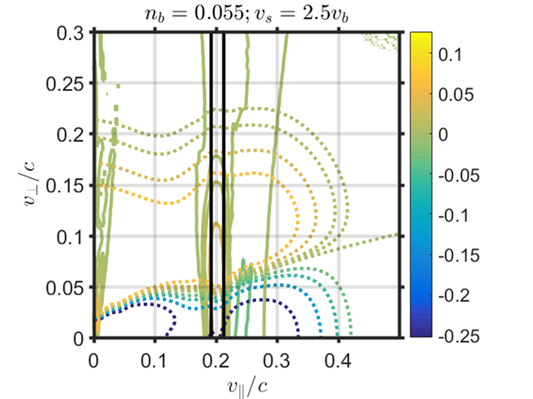
\includegraphics[width=0.5\linewidth]{part3/FR1.png}
\centering
\captionstyle{normal}
\caption{Вычисленные для момента времени $\omega_pt=5000$ линии уровня нормированной на максимум начального распределения поправки к пространственно однородной компоненте функции распределения электронов по скоростям (\ref{eq:bp}), которая в начальный момент времени являлась максвелловской с пучком, в случае учета только двухпотоковых мод (сплошная) и в случае совместной эволюции ленгмюровской и вейбелевской турбулентности (пунктир). Параметры начального распределения (4): $n_s=0.055n_b$, $\beta_s=2.5\beta_T$, $\beta_T=0.1$. Вертикальные черные линии выделяют область скоростей электронов, резонансно взаимодействующих с коллинеарными пучку ленгмюровскими модами, являющимися основными энергонесущими в данный момент времени.}
\label{fig:FR1}
\end{figure}

В отсутствие филаментационных мод на интервалах времени, не более чем в 6 раз превышающих время насыщения двухпотоковой неустойчивости, среднеквадратичное электрическое поле ленгмюровских мод находится на примерно постоянном уровне. Включение филаментационных мод приводит к тому, что сразу после окончания экспоненциального роста этих мод с наибольшим инкрементом, означающего начало существенной анизотропной деформации общей функции распределения электронов по скоростям и переход к нелинейной стадии магнитной турбулентности, начинается довольно резкое затухание ленгмюровских волн~(рис.\ref{fig:average1}a). Декремент затухания каждой ленгмюровской моды определяется формой распределения электронов по скоростям только в резонансной для этой моды области. Поскольку с течением времени спектр ленгмюровских волн смещается в коротковолновую область~(рис.\ref{fig:average1}d), то скорость затухания среднеквадратичного электрического поля ленгмюровских мод зависит от промежутка времени между насыщением роста двухпотоковой и филаментационной неустойчивостей, а значит, от амплитуд начальных возмущений электрического и магнитного полей~(иллюстрация дана на рис.\ref{fig:average1}a). При этом среднеквадратичное индукционное электрическое поле филаментационных мод мало в сравнении с полем ленгмюровских мод на протяжении всей эволюции. Аналогично, малым является и среднеквадратичное магнитное поле ленгмюровских мод в сравнении с полем филаментационных.

Как уже сказано выше, вследствие квазилинейного взаимодействия между ленгмюровскими волнами характерное продольное волновое число их спектра $\langle K_\|\rangle$ увеличивается ~(рис.\ref{fig:average1}d). В приводимом примере это увеличение останавливается на уровне около 20\% примерно на временах, на порядок превышающих время насыщения ленгмюровской турбулентности, и почти не зависит от вейбелевской турбулентности. Однако благодаря её влиянию, а именно, квазилинейной деформации области плато в резонансной части пучкового распределения электронов по скоростям,  продольная среднеквадратичная ширина ленгмюровского спектра $\langle \Delta K_\|\rangle$ сужается весьма значительно, примерно в 1.5 раза согласно~рис.\ref{fig:average1}c, вследствие появления довольно быстрого затухания наиболее коротковолновой части этого спектра. Поперечная среднеквадратичная ширина ленгмюровского спектра $\langle \Delta K_\perp\rangle$ меняется слабо, в пределах нескольких процентов.

\begin{figure}[h]
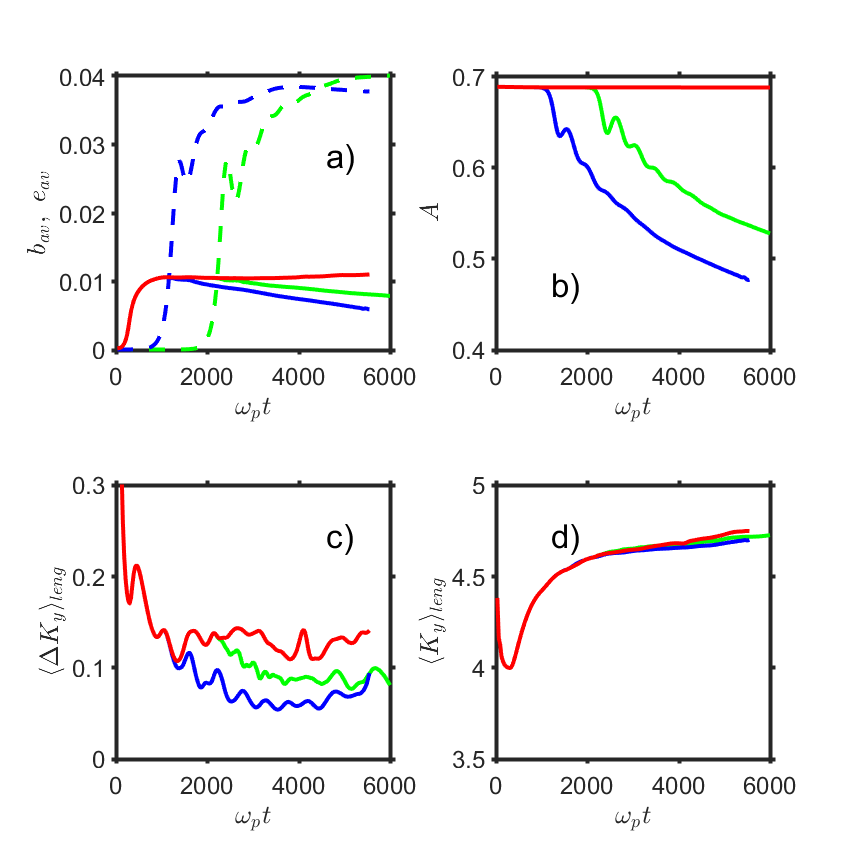
\includegraphics[width=0.5\linewidth]{part3/final_average_v2.png}
\centering
\captionstyle{normal}
\caption{Динамика (a) среднеквадратичного магнитного поля $b_{av}$ филаментационных мод (штрихи) и электрического поля $e_{av}$ двухпотоковых мод (сплошная), (b) параметра анизотропии $A$,  (c) среднеквадратичной ширины спектра ленгмюровских волн вдоль направления пучка $\langle \Delta K_y\rangle$ и (d) их среднеквадратичного продольного волнового числа $\langle K_\|\rangle$  в случае эволюции исключительно двухпотоковых мод (красный цвет) и в случае совместной эволюции двухпотоковых мод и филаментационных мод при уровнях начальных амплитуд последних, отличающихся в $10^4$ раз (синий и зеленый цвета). Параметры начального распределения (\ref{eq:bp}): $n_s=0.055n_b$, $\beta_s=2.5\beta_T$, $\beta_T=0.1$.}
\label{fig:average1}
\end{figure}

Динамика вейбелевской турбулентности, реализующейся на значительно более длинноволновых гармониках, определяется нерезонансным взаимодействием "волна-частица"~\cite{GaleevSagdeev1969,Kuznetsov2023} и слабо чувствительна к форме распределения электронов по скоростям в области резонанса с ленгмюровскими волнами. Ключевым для квазилинейного описания этой турбулентности является интегральный параметр анизотропии $A$, равный отличию от единицы отношения полной энергии электронов в продольном $W_\|$ и поперечном $W_\perp$ к скорости пучка направлении~(\ref{anisotropy}). По мере развития турбулентности распределение электронов изотропизуется, что отражается в монотонном снижении параметра анизотропии~(рис.\ref{fig:average1}b).

В рассматриваемом случае ленгмюровская турбулентность оказывается несущественной для роста флуктуаций магнитного поля и снижение параметра анизотропии диктуется исключительно вейбелевской турбулентностью. На этапе её насыщения это снижение происходит весьма быстро и достигает примерно 30\% от исходной величины $A_0=0.687$. В дальнейшем параметр анизотропии уменьшается значительно медленнее, а спектр вейбелевской турбулентности квазиавтомодельно смещается в длинноволновую область. При этом среднеквадратичное магнитное поле $b_{av}$ непосредственно после окончания экспоненциального роста демонстрирует квазистепенной рост на небольшой    промежуточной стадии, достигает максимума и далее испытывает медленное квазилинейное затухание ~(рис.\ref{fig:average1}a)~\cite{Kuznetsov2023}. В течение всего этого времени магнитная энергия на порядок и более превышает энергию квазиэлектростатического поля.

Такое поведение спектра полностью соответствует полученным ранее результатам квазилинейного подхода к эволюции бимаксвелловского распределения электронов в пределе низкой начальной анизотропии, когда среднее волновое число спектра $\langle K\rangle$ уменьшается примерно по степенному закону~\cite{Kuznetsov2023,Borodachev2016_Radiofiz} . Подобная картина наблюдалась во всех проведенных квазилинейных расчетах для системы "плазма+пучок" с небольшим начальным параметр анизотропии ($A_0\lesssim1$) и высоким уровнем достигаемой магнитной турбулентности по сравнению с ленгмюровской. 

Тем не менее, характеризуя нагрев плазмы, который в данной задаче можно связать с ростом поперечной тепловой энергии электронов $W_\perp$, следует отметить, что он является неравномерным и происходит в три этапа: 1) диссипация квазиэлектростатических полей посредством затухания Ландау в промежутке времени между достижением насыщения ленгмюровской турбулентности и началом насыщения вейбелевской, 2) преимущественная диссипация квазимагнитостатических полей, особенно эффективная в ходе их насыщения, когда амплитуды мод велики и быстро изменяются, создавая наибольшие индукционные электрические поля, 3) более медленная диссипация обоих типов квазистатических полей на временах, значительно превышающих время насыщения магнитной турбулентности. Последний этап на рис.\ref{fig:average1} не показан, а первый этап выражен слабо из-за низкого уровня развившейся ленгмюровской турбулентности. Указанные этапы нагрева имеют место и в ситуации, представленной в следующем разделе, причем там уровень ленгмюровской турбулентности выше и поэтому на первом этапе нагрев значительнее.


\section{Ослабление развития магнитной турбулентности ленгмюровскими модами}

При м\'{е}ньших, чем в предыдущем разделе, значениях скорости пучка инкремент двухпотоковых мод ослабляется и они могут развиваться одновременно с филаментационными модами. Однако тогда последние по-прежнему значительно превышают по амплитуде и подавляют первые, тем более не чувствуя наличие очень слабой ленгмюровской турбулентности. Поэтому обратимся к анализу случая б\'{о}льшего, чем в предыдущем разделе, значения скорости пучка, когда достижимы условия, в которых влияние ленгмюровской турбулентности на филаментационные моды существенно, а вклад той и другой турбулентности в изотропизацию распределения электронов по скоростям, т.е. в уменьшение параметра $A$, оказывается сопоставим.

Именно, примем для пучка примерно вдвое б\'{о}льшую направленную скорость и на порядок меньшую концентрацию частиц $n_s=0.005n_b$, $\beta_s=4\beta_T$, сохраняя небольшую начальную анизотропию $A_0=0.16$ и не слишком большой инкремент двухпотоковых мод, примерно лишь на порядок превосходящий инкремент филаментационных. Согласно~(рис. \ref{fig:average_v4}), как и в предыдущем случае, двухпотоковая неустойчивость раньше достигает насыщения, так как инкремент наиболее неустойчивой моды с продольным волновым числом $K_y\approx 3.2$ суть $\gamma_{L}\approx0.027\omega_p$, в то время как наиболее неустойчивая поперечная филаментационная мода с волновым числом $K_x\approx 0.226$ имеет инкремент $\gamma_W\approx1.27*10^{-3}\omega_p$. В результате формирующаяся ленгмюровская турбулентность деформируют распределение электронов по скоростям в области между фоновой плазмой и пучком (рис.~\ref{fig:fr2}), так что квазилинейные инкременты филаментационных мод заметно понижаются, а уровень насыщения среднеквадратичного магнитного поля вейбелевской турбулентности уменьшается примерно вдвое~(рис. \ref{fig:average_v4}a). Вместе с тем такие спектральные характеристики как среднее волновое число $\langle K\rangle$ и поперечная  $\langle\Delta K_x\rangle$  и продольная $\langle \Delta K_y\rangle$ ширина вейбелевского спектра почти не подвержены влиянию ленгмюровской турбулентности и отличаются не более чем на 1-2\% в расчетах с добавлением двухпотоковых мод и без них. 

\begin{figure}[h]
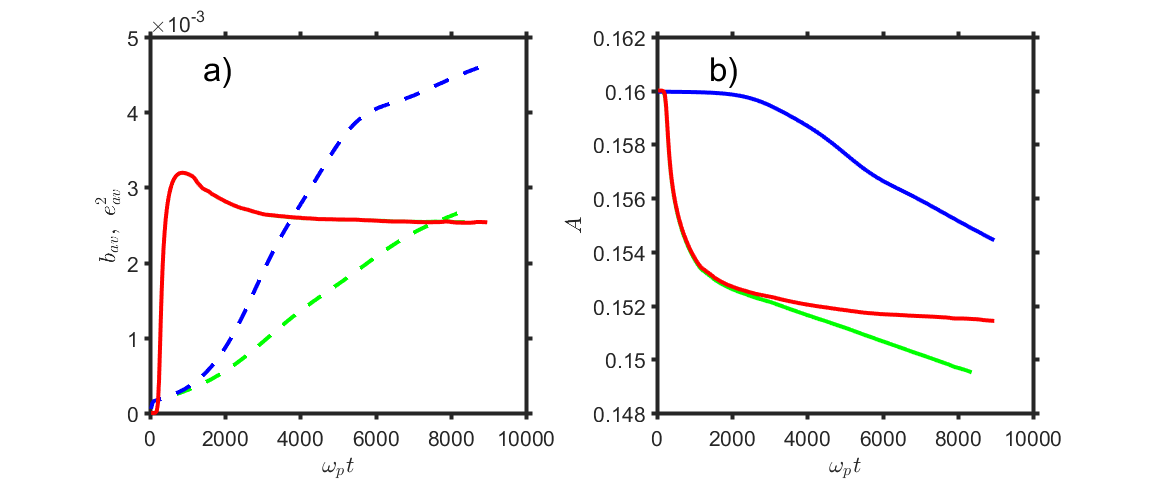
\includegraphics[width=0.7\linewidth]{part3/average_v4.png}
\centering
\captionstyle{normal}
\caption{Динамика (a) среднеквадратичного магнитного поля $b_{av}$ филаментационных мод (штрихи) и среднего квадрата электрического поля $e_{av}^2$ двухпотоковых мод (сплошная), а также (b) параметра анизотропии $A$ в случае эволюции исключительно двухпотоковых (красный цвет) либо филаментационных (синий цвет) мод и в случае их совместной эволюции (зеленый цвет). Параметры начального распределения (\ref{eq:bp}): $n_s=0.005n_b$, $\beta_s=4\beta_T$, $\beta_T=0.1$.} 
\label{fig:average_v4}
\end{figure}

На рассматриваемом промежутке времени дополнительная изотропизация распределения электронов филаментационными модами происходит преимущественно за пределами резонансной с ленгмюровскими волнами области скоростей~(рис.~\ref{fig:fr2}) и фактически начинается только при переходе на стадию насыщения вейбелевской турбулентности при $\omega_p  t > 5000$ (ср. красную и зеленую кривые для параметра анизотропии на рис. \ref{fig:average_v4}b). В результате в расчетах с добавлением филаментационных мод и без них динамика ленгмюровской турбулентности, а именно, её среднеквадратичного электрического поля, характерного волнового числа, поперечной и продольной ширины спектра не отличалась более чем на 10\%. Сказанное не исключает необходимости учета филаментационных мод при анализе затухания ленгмюровских волн на б\'{о}льших временах, на которых, однако, квазилинейное описание может оказаться некорректным из-за нарушения условий его применимости, например, вследствие накопления эффектов нелинейного трёх- или четырёхволнового взаимодействия между отдельными модами.


\begin{figure}[h]
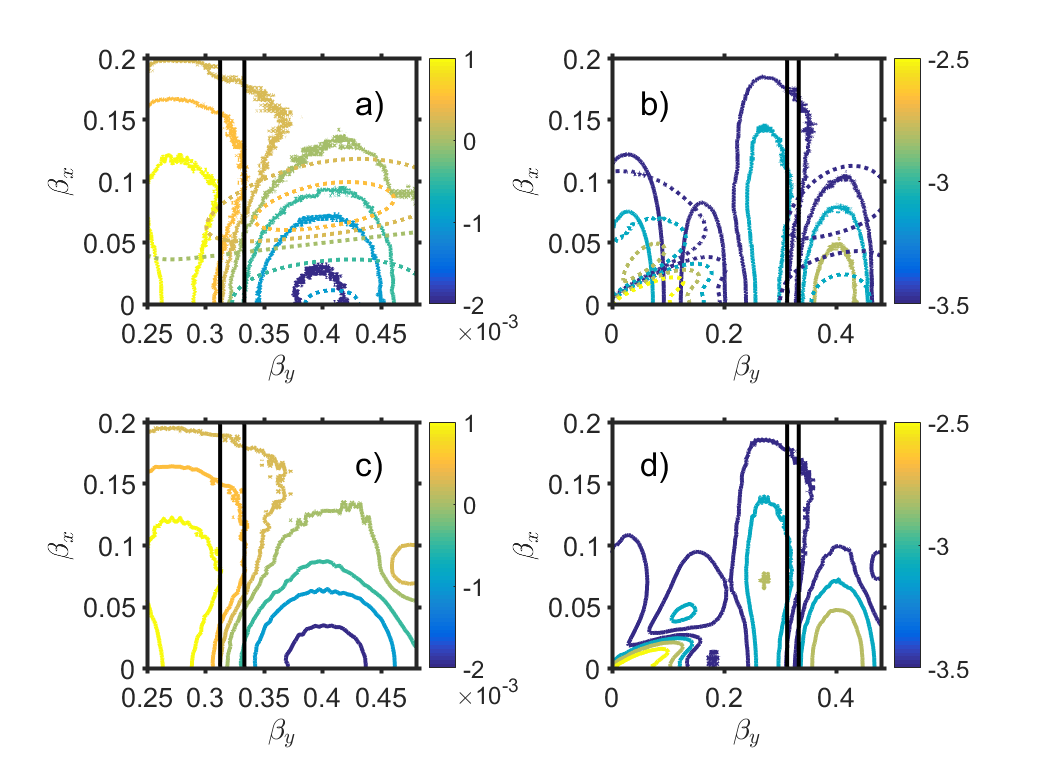
\includegraphics[width=1\linewidth]{part3/fr2.png}
\centering
\captionstyle{normal}
\caption{(a) Вычисленные для момента времени $\omega_pt=8100$ линии уровня нормированной на максимум начального распределения поправки к однородной компоненте функции распределения электронов по скоростям (\ref{eq:bp}), которая в начальный момент времени являлась максвелловской с пучком, в случае учета только двухпотоковых (сплошная) или только филаментационных (пунктир) мод. Параметры начального распределения (\ref{eq:bp}): $n_s=0.005n_b$, $\beta_s=4\beta_T$, $\beta_T=0.1$. Вертикальные черные линии отражают оценку резонансной области для коллинеарных с пучком основных энергонесущих в данный момент времени ленгмюровских мод.(b) То же для десятичного логарифма поправки к однородной компоненте функции распределения. 
(c)-(d) соответствуют графикам (a)-(b) в случае совместного учета двухпотоковых и филаментационных мод.}
\label{fig:fr2}
\end{figure}

По мере дальнейшего увеличения скорости пучка $\beta_s$ уменьшение анизотропии $A$, а также подавление роста филаментационных мод за счет насыщения роста мод ленгмюровского типа становится более значительным. Так, для параметров начального распределения $n_s=0.03n_b$, $\beta_s=5\beta_T$, $\beta_T=0.1$, при которых квазилинейная теория не применима, в расчетах методом частиц в ячейках при помощи кода EPOCH~\cite{Arber2015} турбулентное магнитное поле вейбелевских мод ослабевало примерно на порядок при учете ленгмюровской турбулентности.


\section{Заключение}

Представленные результаты демонстрируют возможные сценарии квазилинейного взаимодействия эволюционирующих спектров ленгмюровской и вейбелевской турбулентности в бесстолкновительной незамагниченной нерелятивистской плазме, включающей фоновую плазму и теплый пучок, в которых начальное распределение электронов является максвелловским с одной и той же температурой, а ионы предполагаются холодными и динамически пассивными. Реализующийся сценарий зависит от величины направленной скорости пучка и отношения концентрации его частиц к концентрации частиц фоновой плазмы. 

Если эта скорость хотя бы в несколько раз превышает тепловую, то в типичных условиях даже при относительно небольшой концентрации пучка инкремент плазменных волн значительно превышает инкремент филаментационной неустойчивости и поэтому ленгмюровская турбулентность коротковолновых квазиэлектростатических полей формируется намного раньше вейбелевской  турбулентности более длинноволновых квазимагнитостатических токов. В этом случае, как показывают квазилинейные расчеты, ленгмюровская турбулентность, выполаживающая функцию распределения электронов по скоростям в области между пучком и фоновой плазмой, может заметно уменьшить величину параметра анизотропии $A$ общего распределения электронов по скоростям, а следовательно, замедлить экспоненциальный рост филаментационных мод, понизить уровень их насыщения в ходе дальнейшего развития неустойчивости и изменить эволюцию спектра. Однако ленгмюровская турбулентность не способна подавить развитие филаментационной турбулентности, хотя результирующая энергия её магнитного поля значительно, как правило многократно, уступает энергии энергии квазиэлектростатического поля ленгмюровской турбулентности. Более того, темп затухания этой турбулентности существенно ускоряется, а расширение её спектра существенно ограничивается в результате квазилинейного воздействия развитой магнитной турбулентности.

Если же направленная скорость пучка не намного превышает тепловую скорость, примерно вдвое или менее, то при относительно небольшой концентрации пучка инкремент ленгмюровских мод оказывается меньше или порядка инкремента филаментационных, так что ленгмюровская турбулентность даже не успевает развиться до уровня собственного насыщения и довольно быстро подавляется нарастающей магнитной турбулентностью. Это происходит во многом благодаря квазилинейному эффекту деформации, сглаживания функции распределения электронов в той области скоростей, где имеет место их резонанс с ленгмюровскими волнами. Иными словами, филаментационная турбулентность квазилинейным образом подавляет ленгмюровскую. 

Проведенный анализ квазилинейного взаимодействия ленгмюровской и вейбелевской турбулентности важен для выявления других механизмов взаимного влияния турбулентных спектров квазиэлектростатических и квазимагнитостатических флуктуаций в плазменно-пучковых системах. Так, в дополнение к исследованиям трехволнового и четырехволнового взаимодействия мод ленгмюровской~\cite{Kasaba2001,Ziebell2008} и вейбелевской ~\cite{Garasev2021,Kuznetsov2025} турбулентности по отдельности, интерес представляет комбинационное взаимодействие филаментационных и двухпотоковых мод. В частности, оно может оказаться существенным для процесса аномального рассеяния резонансных с ленгмюровской волной электронов на флуктуациях магнитного поля~\cite{Fleishman2013,Medvedev2017}. При больших уровнях насыщения той или иной турбулентности, когда она уже не является достаточно слабой, многообещающим является анализ конкуренции квазилинейного взаимодействия двух типов турбулентности с их нелинейным взаимодействием за счет влияния квазиэлектро- и квазимагнитостатических полей на динамику имеющихся локализованных образований, а именно, влияния флуктуаций электрического поля на токовые z-пинчи и влияние флуктуаций магнитного поля на ленгмюровские солитоны. Кроме того, особый интерес вызывает роль аномальных столкновений, обусловленных рассеянием электронов на турбулентности в бесстолкновительной плазме и тоже являющихся нелинейным механизмом изменения инкрементов ленгмюровских и филаментационных мод, а следовательно, механизмом взаимного влияния спектров той и другой турбулентности.  

Наконец, существенным фактором развития и взаимовлияния указанных турбулентных спектров являются обычно имеющееся различие температур фона и пучка и возможное наличие релятивистских частиц в них, игнорировавшиеся в настоящей работе. Так, различие температур фона и пучка допускает пространственное разделение заряда, надлежащий учет которого снижает инкремент филаментационных мод и уровень насыщения магнитной турбулентности~\cite{Tzoufras2006,Hao2008}. 
Для широкого класса релятивистских распределений частиц по скоростям наиболее неустойчивы наклонные моды, у которых угол между волновым вектором и пучком существенно отличен и от $0$, и от $90$ градусов~\cite{Bret2004,Bret2010}. Эти и другие факторы могут повлиять на квазилинейное взаимодействие различных типов турбулентности и заслуживают дальнейшего исследования. В астрофизических задачах учет тех или иных нелинейных факторов, дополняющих разработанное квазилинейное описание совместного развития ленгмюровской и вейбелевской турбулентности, определяется свойствами неравновесной магнитоактивной плазмы конкретных космических объектов и выходит за рамки настоящей работы.
